\documentclass[12pt]{article}
% ----------------------------------------------------------------------
% Define external packages, language, margins, fonts, new commands 
% and colors
% ----------------------------------------------------------------------
\usepackage[utf8]{inputenc} % Codification
\usepackage[english]{babel} % Writing idiom

\usepackage[export]{adjustbox} % Align images
\usepackage{amsmath} % Extra commands for math mode
\usepackage{amssymb} % Mathematical symbols
\usepackage{anysize} % Personalize margins
    \marginsize{2cm}{2cm}{2cm}{2cm} % {left}{right}{above}{below}
\usepackage{appendix} % Appendices
\usepackage{cancel} % Expression cancellation
\usepackage{caption} % Captions
    \captionsetup{labelfont={bf}}
\usepackage{cite} % Citations, like [1 - 3]
\usepackage{color} % Text coloring
\usepackage{fancyhdr} % Head note and footnote
    \pagestyle{fancy}
    \fancyhf{}
    \fancyhead[L]{
        
\includegraphics[scale = 0.4]{NovaFct.png}
    } % Left of Head note
    \fancyhead[R]{\footnotesize Eletrónica para Micro-Sistemas} % Right of Head note
    \fancyfoot[L]{\footnotesize MEEC/MIEEC} % Left of Footnote
    \fancyfoot[R]{\thepage  } % Center of Footnote
    %\fancyfoot[R]{\footnotesize Degree} % Right of Footnote
    \renewcommand{\footrulewidth}{0.4pt} % Footnote rule
\usepackage{float} % Utilization of [H] in figures
\usepackage{graphicx} % Figures in LaTeX
\usepackage[colorlinks = true, plainpages = true, linkcolor = novablue, urlcolor = novablue, citecolor = novablue, anchorcolor = novablue]{hyperref}
\usepackage{indentfirst} % First paragraph
\usepackage[super]{nth} % Superscripts
\usepackage{siunitx} % SI units
\usepackage{subcaption} % Subfigures
\usepackage{titlesec} % Font
    \titleformat{\section}{\Large\bfseries}{\thesection}{1em}{}
    \titleformat{\subsection}{\large\bfseries}{\thesubsection}{1em}{}
    \titleformat{\subsubsection}{\normalsize\bfseries}{\thesubsubsection}{1em}{}
    %\fancyfoot[C]{\thepage}

%code
\usepackage[breakable]{tcolorbox}

% Code highlighting
\usepackage{listings}
\lstset{ 
    backgroundcolor=\color{cellbackground}, % background color for the code block
    basicstyle=\ttfamily,                   % font style
    breakatwhitespace=false,                % automatic breaks only at whitespace
    breaklines=true,                        % automatic line breaking
    captionpos=b,                           % caption position
    commentstyle=\color{gray},              % comment style
    escapeinside={\%*}{*)},                 % if you want to add LaTeX within your code
    keywordstyle=\color{blue},              % keyword style
    stringstyle=\color{dkgreen},            % string style
    frame=single,                           % adds a frame around the code
    rulecolor=\color{cellborder},           % border color
}

% Exact colors from NB
\definecolor{incolor}{HTML}{303F9F}
\definecolor{outcolor}{HTML}{D84315}
\definecolor{cellborder}{HTML}{CFCFCF}
\definecolor{cellbackground}{HTML}{F7F7F7}

% Random text (not needed)
\usepackage{lipsum}
\usepackage{duckuments}

% New and re-newcommands
\newcommand{\sen}{\operatorname{\sen}} % Sine function definition
\newcommand{\HRule}{\rule{\linewidth}{0.5mm}} % Specific rule definition
\renewcommand{\appendixpagename}{\LARGE Appendices}

% Colors
\definecolor{novablue}{RGB}{0, 101, 189}
\definecolor{dkgreen}{rgb}{0,0.6,0}
\definecolor{gray}{rgb}{0.5,0.5,0.5}

%%%%%%%%%%%%%%%%%%%%%%%%%%%%%%%%%%%%%%%%%%%%%%%%%%%%%%%%%%%%%%%%%%%%%%%%
%                                 Document                             %
%%%%%%%%%%%%%%%%%%%%%%%%%%%%%%%%%%%%%%%%%%%%%%%%%%%%%%%%%%%%%%%%%%%%%%%%
\begin{document}

% ----------------------------------------------------------------------
% Cover
% ----------------------------------------------------------------------
\begin{center}
    \begin{figure}
        \vspace{-1.0cm}
        
\includegraphics[scale = 1, left]{NovaFct.png} % Nova logo
    \end{figure}

    \mbox{}\\[2.0cm]
    \textsc{\Huge MEEC/MIEEC}\\[2.5cm]
    \textsc{\LARGE Electronics for Micro-Systems}\\[2.0cm]
    \HRule\\[0.4cm]
    {\large \bf { Lab\#1 P1\linebreak A Temperature Meter
    System with 3 Sensors,
    Relay and GUI
    }}\\[0.2cm] % [\texttt{EN}]
    \HRule\\[1.5cm]
\end{center}

\begin{flushleft}
    \textbf{Authors:}
\end{flushleft}

\begin{center}
    \begin{minipage}{0.5\textwidth}
        \begin{flushleft}
            Martim Duarte Agostinho (70392)\\
            Francisco Simões Coelho Sá da Costa   (\texttt{70386})\\
            Sofia Margarida Mafra Dias Inácio (58079)\\
        \end{flushleft}
    \end{minipage}%
    \begin{minipage}{0.5\textwidth}
        \begin{flushright}
            \href{mailto:md.agostinho@campus.fct.unl.pt}{\texttt{md.agostinho@campus.fct.unl.pt}}\\
            \href{mailto:fsc.costa@campus.fct.unl.pt}{\texttt{fsc.costa@campus.fct.unl.pt}}\\
            \href{mailto:sm.inacio@campus.fct.unl.pt}{\texttt{sm.inacio@campus.fct.unl.pt}}
        \end{flushright}
    \end{minipage}
\end{center}
 
% Caixa a dizer o grupo
%\begin{flushleft}
%    \large $\boxed{\text{\bf Group} \ \clubsuit}$\\[4.0cm]
%\end{flushleft}

\vspace{6cm}

\begin{center}
    \large \bf 2024/2025 -- \nth{1} Semester -- DEEC
\end{center}

\thispagestyle{empty}

\setcounter{page}{0}

\newpage

\newpage

\tableofcontents % Generates the table of contents

\newpage

\listoffigures

\newpage

\section{Introduction}
explain the requirements and the main objectives of the project
\textcolor{red}{
    Se calhar dizer aqui quais sao as metricas por onde podemos avaliar a nossa solucao
    Linearidade de output para conseguir aproveitar melhor a resolucao do adc 
    Consumo
    erro}

    \begin{figure}[H] 
        \centering
        \includegraphics*[scale = 0.5]{images/system-design.png}
        \caption{Temperature sensing system with 3 three types of sensors.}
        \label{wrap-fig:1}
    \end{figure}

\pagebreak

\section{Temperature Sensors}
\subsection{NTC - Negative Temperature Coefficient}

\subsection{LM35 - Precision Centigrade Temperature Sensor}

\subsection{DS18B20 - Digital Thermometer}

\section{System Design}
\subsection{Analog FrontEnd (AFE) NTC}
\label{ AFENTC }

    \textcolor{red}{A parte onde definimos o intervalo de temperatura nao devia estar aqui pq é para todos os circuitos}


    In order to design the \textit{NTF} \textit{AFE} first it's necessary to define the temperature interval
    in which this circuit will work, thus it was define as $T \in [ 10^{\circ}; 40^{\circ} ]$. 
    Through the \textit{NTC}'s datasheet the interval of its resistance values is $R_{NTC} \in [~5,282k~;~19,98k~]$

    For an accurate reading of the temperature it was used the 
    \hyperref[eq:1]{ \textit{Steinhart-Hart} equation}.

    \begin{equation} \label{eq:1}
    \frac{1}{T} = A + B\cdot \ln(R_{NTC}) + C\cdot [\ln(R_{NTC})]^3
    \end{equation}

    In order to find the parameters $A$, $B$ and $C$, its necessary to use 3 points from the datasheet. 
    The points chosen were the two extremes and the middle point.

    \begin{equation}
        \begin{cases}
        
            R( 283,15 ) = 1,998\cdot 10^4 ~\Omega \\
            R( 298,15 ) = 10^4 ~\Omega\\
            R( 313,15 ) = 0,5282 \cdot 10^4 ~\Omega\\
        
        \end{cases}
        \Leftrightarrow
        \begin{cases}
            A = 1,2 \cdot 10^{-3}\\
            B = 2,1 \cdot 10^{-4}\\
            C = 1,3 \cdot 10^{-7}\\
        
        \end{cases}
    \end{equation}

    The simplest way to convert the resistance to voltage, is to use a voltage divider circuit.


   \begin{figure}[H] 
        \centering
        \includegraphics*[scale = 0.25]{images/voltagedivider.png}
        \caption{NTC voltage divider.}
        \label{wrap-fig:1}
    \end{figure}

    This approach  has a few problems: 

    $\cdot$ The output resistance is really high $R\parallel NTC$, 

    $\cdot$ The output voltage is highly non linear, which is a problem because this way some \textit{ADC} resolution is lost.

    The first problem is solved through a buffer at the entrance of the \textit{AFE}, 
    and the second is somewhat mitigated by using a resistor value around $8K \Omega$.
    To achieve this value it was used the beta model for the $NTC$ and through a python script,
    the resistor value was iterated until an almost linear output was achieved. 
    See NtcTempToVoltage() function in the attached python script.  
    
    \begin{figure}[h]
        \centering
        \begin{subfigure}{0.45\textwidth}
            \centering
            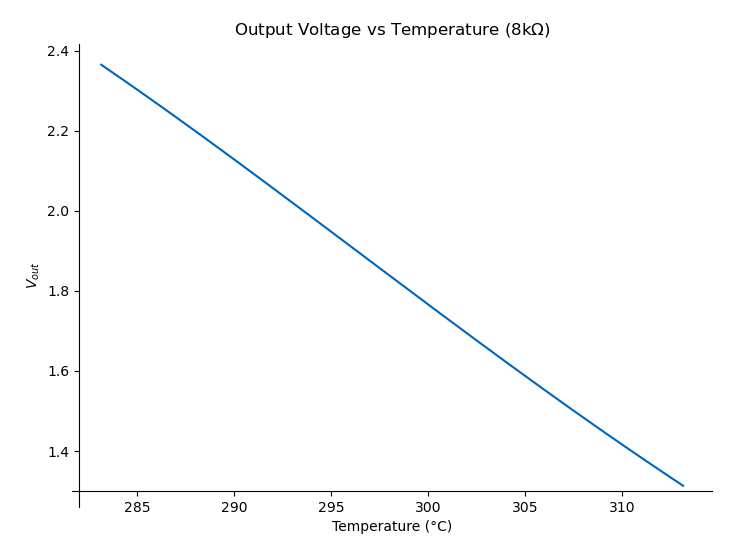
\includegraphics[width=\textwidth]{images/VoutPorTemp.png}
            \caption{ $8K\Omega$ }
        \end{subfigure}\hfill
        \begin{subfigure}{0.45\textwidth}
            \centering
            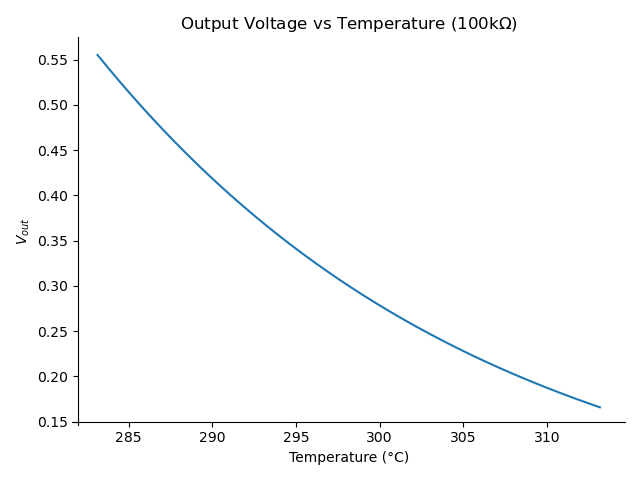
\includegraphics[width=\textwidth]{images/VoutPorTemp100k.png}
            \caption{$100K\Omega$}
        \end{subfigure}
        \caption{Output Voltage vs Temperature}
    \end{figure}


    With $R=8k$ the output signal is $V_{out} \in [1.31V;2.36V]$. 
    But the \textit{ADC} as resolution of $12$ bits and a voltage range of $3.3V$, meaning that to have the best resolution possible the signal needs an offset and a gain of $2.87$ and $-1.75$ respectively. 
    It's important to note that a $0.1V$ margin was added to $V_{out}$ in order to ensure that the \textit{AFE} works properly in the specified range.
    
    The most obvious way to achieve this values would be with a differential amplifier, 
    as seen in the following circuit.

     \begin{figure}[H] 
        \centering
        \includegraphics*[scale = 0.25]{images/AFENTCDiffAmp.png}
        \caption{NTC's AFE Differential Amplifier}
        \label{wrap-fig:1}
    \end{figure}

    Although in the simulation this yields the expected result buy using the 
    
    This gain and offset was achieved through the following topology.
    
    \begin{figure}[H] 
        \centering
        \includegraphics*[scale = 0.25]{images/AFENTC.png}
        \caption{NTC's AFE topology}
        \label{wrap-fig:1}
    \end{figure}

    \textcolor{red}{Nao esquecer de fazer referencia ao codigo funcao AfeNtc()}

    As already specified the $R_3$ value is $8K~\Omega$ and for the purpose circuit dimensioning the circuit 
    the positive node of the opamp will be treated as a variable $V_p$.

    Using python the circuit function $V_{out}(V_p)$:
    
    \begin{equation}
        V_{out} = V_p\left[ 1 + R_f\cdot\left(\frac{1}{R_1} + \frac{1}{R_2}\right) \right] - V_{cc}\cdot\frac{R_f}{R_1}
    \end{equation}

    Now it's clear to see what part of the equation is responsible for the circuit gain and offset.
    
    \begin{equation}
        \begin{cases}
            V_{offset} = - V_{cc}\cdot\frac{R_f}{R_1}\\
            G = \left[ 1 + R_f\cdot\left(\frac{1}{R_1} + \frac{1}{R_2}\right) \right]\\
        \end{cases}
    \end{equation}

    Setting $R_f = 10K$ the values that satisfy the equation system are $R_1 = 9348 \Omega$ and $R_2 = 11760 \Omega$.
    In the simulation this values are a bit too close to the limits so in order to have better margins and to use the available resistors
    the final values are  $R_1 = 8.2K \Omega$ and $R_2 = 12K \Omega$.

    

\subsection{LM35}

    This integrated-circuit temperature sensor, generates an output
    voltage linearly proportional to the Centigrade temperature.

    $$V_{out} = 10^{-2}\cdot T$$

    Hence, in the specified conditions $V_{out}\in[0.1;0.4]$. 
    To increase resolution as done in \hyperref[ AFENTC ]{NTC's AFE subsection},
    it's needed to add gain and an offset. 
    For this purpose a differential amplifier can be used.  
    
    \begin{figure}[H] 
        \centering
        \includegraphics*[scale = 0.3]{images/DiffAmpLM35.png}
        \caption{LM35 Differential Amplifier.}
        \label{wrap-fig:1}
    \end{figure}

    Although this circuit achieves the expected output, the amount of components,
    increases noise and power consumption, thus the used topology was a non-inverting amplifier.

    \begin{figure}[H] 
        \centering
        \includegraphics*[scale = 0.2]{images/AFELM35.png}
        \caption{AFE for the LM35 sensor.}
        \label{AFELM35}
    \end{figure}

    FALTA DIZER O GANHO COM A RES REAL
    This way the input impedance is high, only one OpAmp and two resistors are used.
    But this comes with the cost of lost resolution. With a gain of $8$ $V_{out}\in[0.8V,3.2V]$
    $0.8V$ or $24\%$ of range in the \textit{ADC} are lost.

\subsection{Output Relay }
    
    Lastly the \textit{MCU} will turn on and off a fan. For this purpose 
    a relay will open and close the fan circuit. Because the \textit{MCU's I/O} 
    can't drive the relay a \textit{NPN} transistor is use to get enough current.
    Thus the following circuit also needs to be dimensioned. It's important to note
    that the diode is needed to protect the circuit.
    
    \begin{figure}[H] 
        \centering
        \includegraphics*[scale = 0.4]{images/RelayDrive.png}
        \caption{Relay circuit.}
        \label{wrap-fig:1}
    \end{figure}
    \textcolor{red}{PRECISA DE ENCHER CHOURICO AQUI}
    \begin{equation}
        R = \frac{I/O_{HIGH}-V_{BE}}{I_r}\cdot \beta\\
        \Leftrightarrow R = 
    \end{equation}


\newpage
\section{Simulations}
\subsection{NTC}
    
    For the purpose of testing the following circuit was designed.
    At first with linear voltage supply since as seen in \hyperref{AFENTC}{NTC's AFE} section, this voltage is almost linear.

    Producing the following results.
 
    \begin{figure}[H] 
        \centering
        \includegraphics*[scale = 0.3]{images/NTCLinearRes.png}
        \caption{Linear supply NTC test results.}
        \label{wrap-fig:1}
    \end{figure}

    Confirming the effectiveness of the \textit{AFE} circuit a more realistic
    circuit was then tested.

    \begin{figure}[H] 
        \centering
        \includegraphics*[scale = 0.45]{images/NTCRealTb.png}
        \caption{Realistic NTC test circuit.}
        \label{wrap-fig:1}
    \end{figure}
    
    With the following results.
    
    \begin{figure}[H] 
        \centering
        \includegraphics*[scale = 0.3]{images/NTCRealRes.png}
        \caption{Realistic NTC test results.}
        \label{wrap-fig:1}
    \end{figure}

    \textcolor{red}{Nao gostei de como ficou a frase }
    
    Comparing both results the difference is minimal.
    Confirming that the output is nearly linear in relation to the temperature variation.
    
    \begin{figure}[H] 
        \centering
        \includegraphics*[scale = 0.3]{images/NTCRealLinearComp.png}
        \caption{NTC Linear and Realistic results comparison.}
        \label{wrap-fig:1}
    \end{figure}


\subsection{LM35}

    For this sensor the simulation is straight forward, since the output is linear and proportional to the temperature, 
    it can be simulated with a variable voltage supply. 
    
    The circuit used to test was the same seen in the \hyperref[AFELM35]{lm35 design section}.
    Giving the following results, confirming that this approach works as expected. 
    
    \begin{figure}[H] 
        \centering
        \includegraphics*[scale = 0.15]{images/LM35AFERes.jpeg}
        \caption{LM35 AFE test results.}
        \label{wrap-fig:1}
    \end{figure}

\subsection{Monte-Carlo Analysis} 
    
    The Monte-Carlo simulation is needed for the sake of testing our circuits results variation with the true values of the resistances considering 
    the normal distribuition of thus values. 

    This values can be written by the following expression.
    \begin{equation}
        R_{real} = R_{ideal} * (1 \pm tol)
    \end{equation}
    Where the varaible \textit{tol} will depend with the serie of resistances used. 
    In this work, the serie used is the E12, with a maximum tolerance of 5. So to test the results of
    the output of the two AFE circuits, thirty simulations were made to assure the reliability of the normal distribuition.

    The results for the NTC AFE are the following.

    \begin{figure}[H]
        \centering
        \includegraphics*[scale = 0.3]{images/montecarlo ntc.png}
        \caption{NTC AFE Monte-Carlo test results}
        \label{wrap-fig:1}
    \end{figure}

    And the results for the LM35 AFE circuits.

    \begin{figure}[H]
        \centering
        \includegraphics*[scale = 0.3]{images/montecarlo lm35.png}
        \caption{LM35 AFE Monte-Carlo test results}
        \label{wrap-fig:1}
    \end{figure}

    By analysing the results of the Monte-Carlo simulation of the NTC AFE, firts of all, we can conclude that the
    slope of the output voltage will be almost the same, the only diference will be in the offset of this function.
    This variation on the offset will unfortunally alter the final result for all temperatures, but the maximum diviation is just 3ªC, in a worts case senario.

    One other implication of this offset is the values for lower temperatures, where the output would be greater than 3.3V, so the OpAmp will saturate and the voltage will stay at 3.3V.

    For the results of the LM35 AFE Monte-Carlo test, the biggest diference between the thirty simulations is the slope of the output voltage,
    because the resistances in this circuit only affects it's gain. This consequence is more problematic at higher temperatures, since the input voltage is greater at this values.
\section{Implementation and Experimental Tests}

\section{Results Analysis}

\section{Conclusion}

\end{document}